\documentclass{standalone}
\usepackage{tikz}
\usetikzlibrary{patterns, positioning}
\usepackage[sfdefault]{ClearSans} %% option 'sfdefault' activates Clear Sans as the default text font
\usepackage[T1]{fontenc}

\begin{document}
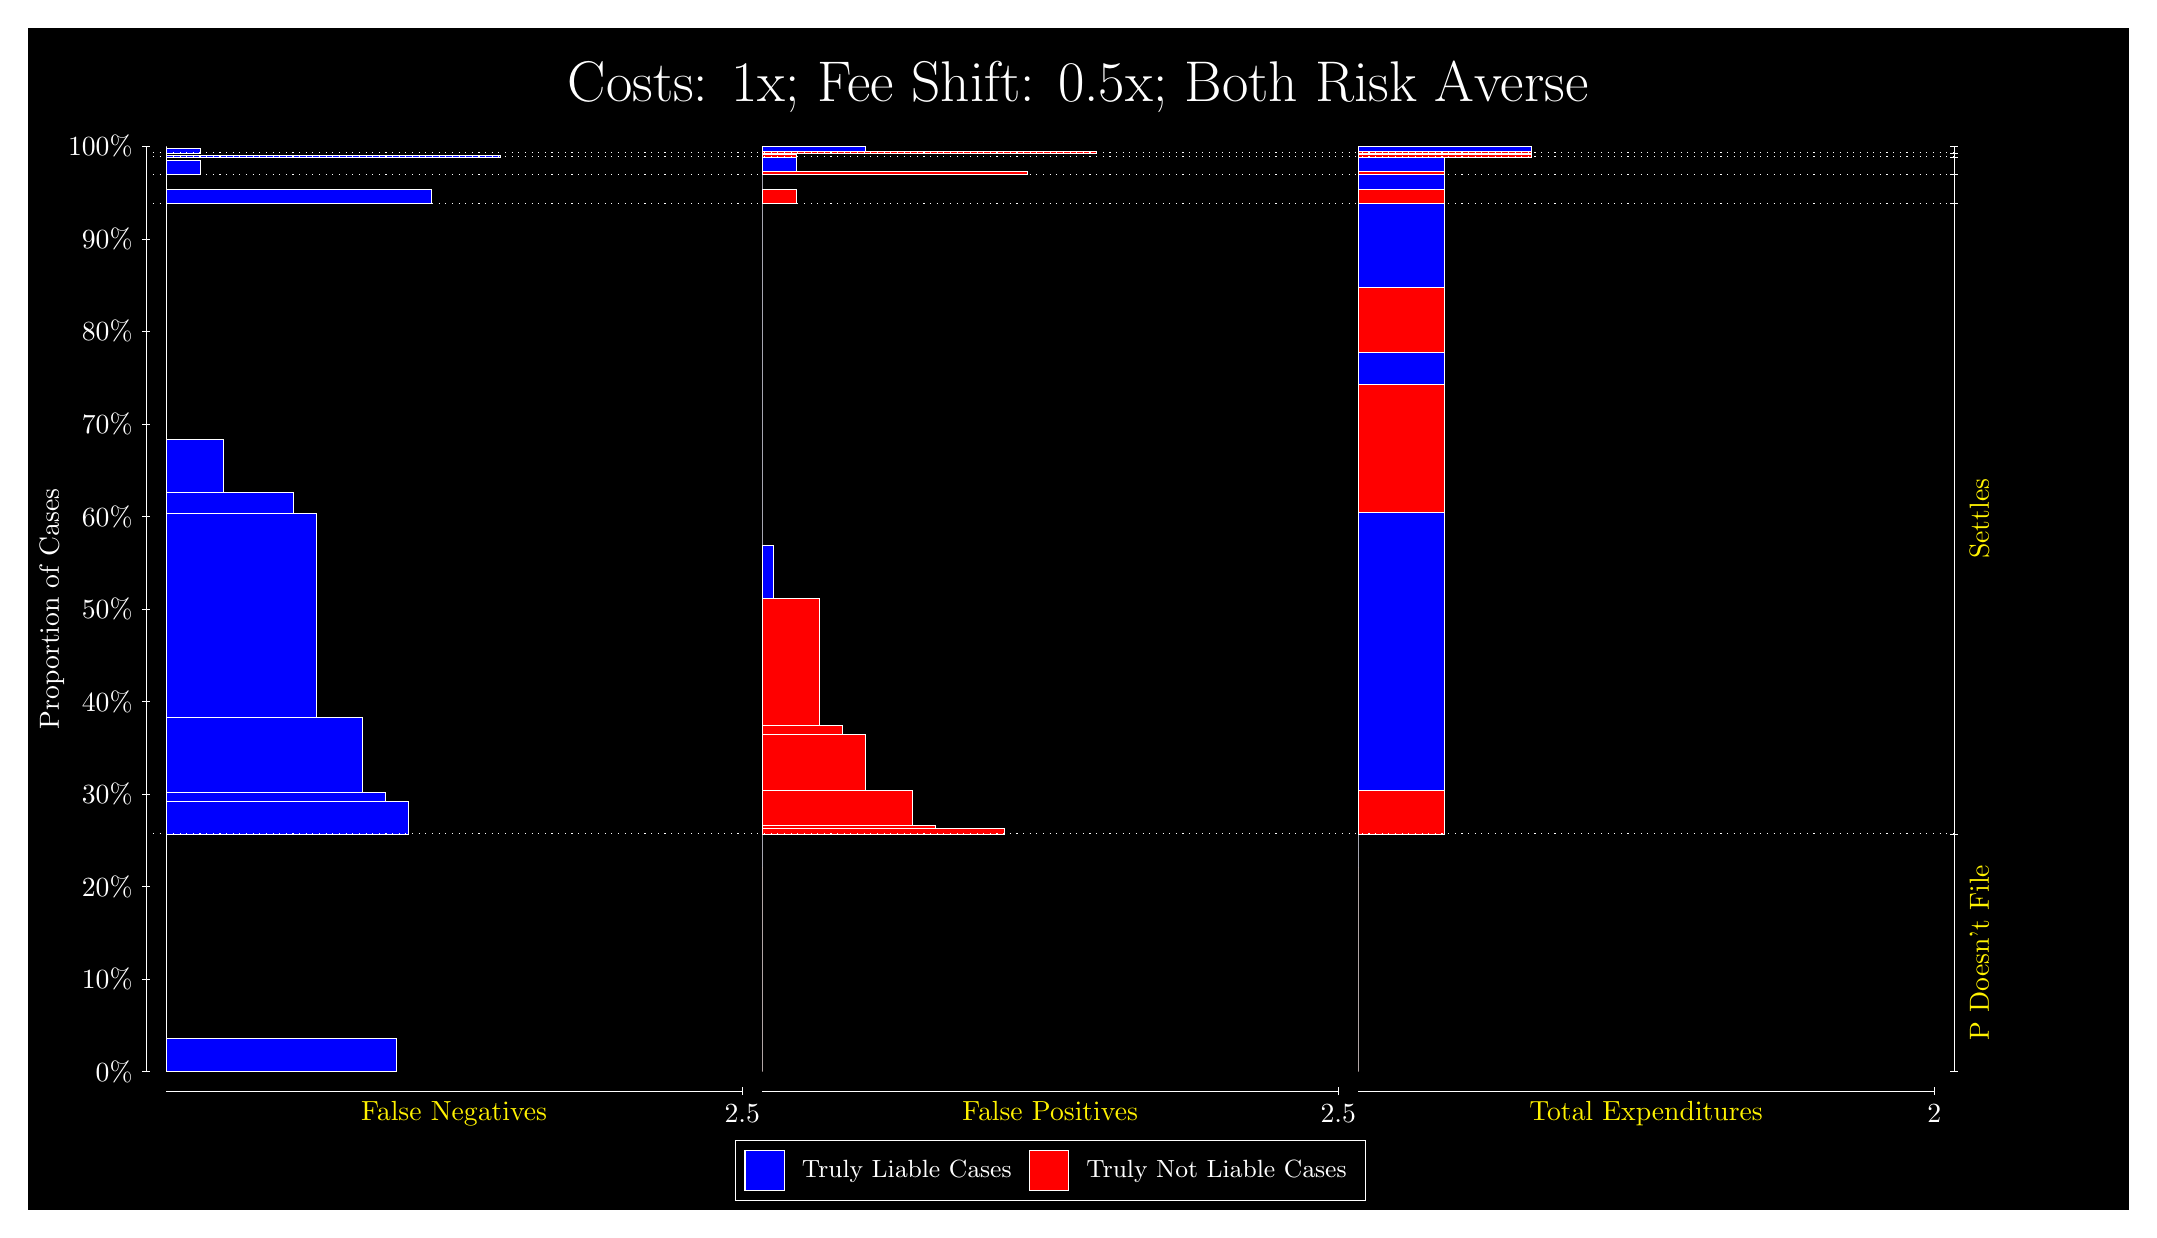
\begin{tikzpicture}
\draw[fill=black] (0,0) rectangle (26.667,15);
\draw[text=white] (0,13.5) rectangle (26.667,15) node[midway] {\huge Costs: 1x; Fee Shift: 0.5x; Both Risk Averse};
\draw[white, very thin] (1.5,1.75) -- (1.5,13.5);
\node[rotate=90, text=white, anchor=center] at (0.3, 7.625) {Proportion of Cases};
\draw[white, very thin] (1.45,1.75) -- (1.55,1.75);
\node[text=white, anchor=east] at (1.45, 1.75) {0\%};
\draw[white, very thin] (1.45,2.925) -- (1.55,2.925);
\node[text=white, anchor=east] at (1.45, 2.925) {10\%};
\draw[white, very thin] (1.45,4.1) -- (1.55,4.1);
\node[text=white, anchor=east] at (1.45, 4.1) {20\%};
\draw[white, very thin] (1.45,5.275) -- (1.55,5.275);
\node[text=white, anchor=east] at (1.45, 5.275) {30\%};
\draw[white, very thin] (1.45,6.45) -- (1.55,6.45);
\node[text=white, anchor=east] at (1.45, 6.45) {40\%};
\draw[white, very thin] (1.45,7.625) -- (1.55,7.625);
\node[text=white, anchor=east] at (1.45, 7.625) {50\%};
\draw[white, very thin] (1.45,8.8) -- (1.55,8.8);
\node[text=white, anchor=east] at (1.45, 8.8) {60\%};
\draw[white, very thin] (1.45,9.975) -- (1.55,9.975);
\node[text=white, anchor=east] at (1.45, 9.975) {70\%};
\draw[white, very thin] (1.45,11.15) -- (1.55,11.15);
\node[text=white, anchor=east] at (1.45, 11.15) {80\%};
\draw[white, very thin] (1.45,12.325) -- (1.55,12.325);
\node[text=white, anchor=east] at (1.45, 12.325) {90\%};
\draw[white, very thin] (1.45,13.5) -- (1.55,13.5);
\node[text=white, anchor=east] at (1.45, 13.5) {100\%};

\draw[white, very thin] (24.457,1.75) -- (24.457,13.5);
\draw[white, very thin] (24.407,1.75) -- (24.507,1.75);
\node[anchor=west] at (24.407, 1.75) {};
\draw[white, very thin] (24.407,4.7682) -- (24.507,4.7682);
\node[anchor=west] at (24.407, 4.7682) {};
\draw[white, very thin] (24.407,12.773) -- (24.507,12.773);
\node[anchor=west] at (24.407, 12.773) {};
\draw[white, very thin] (24.407,13.141) -- (24.507,13.141);
\node[anchor=west] at (24.407, 13.141) {};
\draw[white, very thin] (24.407,13.366) -- (24.507,13.366);
\node[anchor=west] at (24.407, 13.366) {};
\draw[white, very thin] (24.407,13.417) -- (24.507,13.417);
\node[anchor=west] at (24.407, 13.417) {};
\draw[white, very thin] (24.407,13.5) -- (24.507,13.5);
\node[anchor=west] at (24.407, 13.5) {};

\draw[white, very thin, fill=blue] (1.75,1.75) rectangle (4.6775,2.172);
\draw[white, very thin, fill=red] (1.75,2.172) rectangle (1.75,4.7682);
\draw[white, very thin, fill=blue] (1.75,4.7682) rectangle (4.8239,5.1762);
\draw[white, very thin, fill=blue] (1.75,5.1762) rectangle (4.5312,5.2989);
\draw[white, very thin, fill=blue] (1.75,5.2989) rectangle (4.2384,6.2445);
\draw[white, very thin, fill=blue] (1.75,6.2445) rectangle (3.6529,8.8355);
\draw[white, very thin, fill=blue] (1.75,8.8355) rectangle (3.3602,9.1099);
\draw[white, very thin, fill=blue] (1.75,9.1099) rectangle (2.4819,9.7762);
\draw[white, very thin, fill=red] (1.75,9.7762) rectangle (1.75,12.773);
\draw[white, very thin, fill=blue] (1.75,12.773) rectangle (5.1167,12.956);
\draw[white, very thin, fill=red] (1.75,12.956) rectangle (1.75,13.141);
\draw[white, very thin, fill=blue] (1.75,13.141) rectangle (2.1891,13.32);
\draw[white, very thin, fill=red] (1.75,13.32) rectangle (1.75,13.366);
\draw[white, very thin, fill=blue] (1.75,13.366) rectangle (5.9949,13.388);
\draw[white, very thin, fill=red] (1.75,13.388) rectangle (1.75,13.417);
\draw[white, very thin, fill=blue] (1.75,13.417) rectangle (2.1891,13.478);
\draw[white, very thin, fill=red] (1.75,13.478) rectangle (1.75,13.5);
\draw[white, very thin, fill=red] (9.3189,1.75) rectangle (9.3189,4.3462);
\draw[white, very thin, fill=blue] (9.3189,4.3462) rectangle (9.3189,4.7682);
\draw[white, very thin, fill=red] (9.3189,4.7682) rectangle (12.393,4.8354);
\draw[white, very thin, fill=red] (9.3189,4.8354) rectangle (11.515,4.8778);
\draw[white, very thin, fill=red] (9.3189,4.8778) rectangle (11.222,5.3204);
\draw[white, very thin, fill=red] (9.3189,5.3204) rectangle (10.636,6.028);
\draw[white, very thin, fill=red] (9.3189,6.028) rectangle (10.344,6.1416);
\draw[white, very thin, fill=red] (9.3189,6.1416) rectangle (10.051,7.7652);
\draw[white, very thin, fill=blue] (9.3189,7.7652) rectangle (9.4652,8.4315);
\draw[white, very thin, fill=blue] (9.3189,8.4315) rectangle (9.3189,12.773);
\draw[white, very thin, fill=red] (9.3189,12.773) rectangle (9.758,12.958);
\draw[white, very thin, fill=blue] (9.3189,12.958) rectangle (9.3189,13.141);
\draw[white, very thin, fill=red] (9.3189,13.141) rectangle (12.686,13.186);
\draw[white, very thin, fill=blue] (9.3189,13.186) rectangle (9.758,13.366);
\draw[white, very thin, fill=red] (9.3189,13.366) rectangle (9.758,13.395);
\draw[white, very thin, fill=blue] (9.3189,13.395) rectangle (9.3189,13.417);
\draw[white, very thin, fill=red] (9.3189,13.417) rectangle (13.564,13.44);
\draw[white, very thin, fill=blue] (9.3189,13.44) rectangle (10.636,13.5);
\draw[white, very thin, fill=red] (16.888,1.75) rectangle (16.888,4.3462);
\draw[white, very thin, fill=blue] (16.888,4.3462) rectangle (16.888,4.7682);
\draw[white, very thin, fill=red] (16.888,4.7682) rectangle (17.986,5.3204);
\draw[white, very thin, fill=blue] (16.888,5.3204) rectangle (17.986,8.8521);
\draw[white, very thin, fill=red] (16.888,8.8521) rectangle (17.986,10.476);
\draw[white, very thin, fill=blue] (16.888,10.476) rectangle (17.986,10.884);
\draw[white, very thin, fill=red] (16.888,10.884) rectangle (17.986,11.705);
\draw[white, very thin, fill=blue] (16.888,11.705) rectangle (17.986,12.773);
\draw[white, very thin, fill=red] (16.888,12.773) rectangle (17.986,12.958);
\draw[white, very thin, fill=blue] (16.888,12.958) rectangle (17.986,13.141);
\draw[white, very thin, fill=red] (16.888,13.141) rectangle (17.986,13.186);
\draw[white, very thin, fill=blue] (16.888,13.186) rectangle (17.986,13.366);
\draw[white, very thin, fill=red] (16.888,13.366) rectangle (19.083,13.395);
\draw[white, very thin, fill=blue] (16.888,13.395) rectangle (19.083,13.417);
\draw[white, very thin, fill=red] (16.888,13.417) rectangle (19.083,13.44);
\draw[white, very thin, fill=blue] (16.888,13.44) rectangle (19.083,13.5);
\draw[white, dotted] (1.5,4.7682) -- (24.457,4.7682);
\draw[white, dotted] (1.5,12.773) -- (24.457,12.773);
\draw[white, dotted] (1.5,13.141) -- (24.457,13.141);
\draw[white, dotted] (1.5,13.366) -- (24.457,13.366);
\draw[white, dotted] (1.5,13.417) -- (24.457,13.417);
\draw[white, very thin] (1.75,1.5) -- (9.0689,1.5);
\node[text=yellow, anchor=north] at (5.4094, 1.5) {False Negatives};
\draw[white, very thin] (9.0689,1.45) -- (9.0689,1.55);
\node[text=white, anchor=north] at (9.0689, 1.45) {2.5};

\draw[white, very thin] (9.3189,1.5) -- (16.638,1.5);
\node[text=yellow, anchor=north] at (12.978, 1.5) {False Positives};
\draw[white, very thin] (16.638,1.45) -- (16.638,1.55);
\node[text=white, anchor=north] at (16.638, 1.45) {2.5};

\draw[white, very thin] (16.888,1.5) -- (24.207,1.5);
\node[text=yellow, anchor=north] at (20.547, 1.5) {Total Expenditures};
\draw[white, very thin] (24.207,1.45) -- (24.207,1.55);
\node[text=white, anchor=north] at (24.207, 1.45) {2};

\node[text=yellow, centered, rotate=90] at (24.777, 3.2591) {P Doesn't File};
\node[text=yellow, centered, rotate=90] at (24.777, 8.7707) {Settles};





\draw (12.978300999999998,1.5) node[draw=none] (baseCoordinate) {};
\begin{scope}[align=center]
        \matrix[scale=0.5, draw=white, below=0.5cm of baseCoordinate, nodes={draw}, column sep=0.1cm]{
            \node[rectangle, draw, minimum width=0.5cm, minimum height=0.5cm, fill=blue] {}; &
            \node[draw=none, font=\small, text=white] (B) {Truly Liable Cases}; &
            \node[rectangle, draw, minimum width=0.5cm, minimum height=0.5cm, fill=red] {}; &
            \node[draw=none, font=\small, text=white] (B) {Truly Not Liable Cases}; \\
            };
\end{scope}

\end{tikzpicture}
\end{document}